\section{Calibration Against Experiment}\label{sec:calibration}

\subsection{Inputs, targets and the estimator}
\label{sec:controls}\label{sec:targets}\label{sec:objective}

The formulation of \cref{sec:formulation} contains several classes of input, and
confusing them is the commonest way to misreport a calibration.
\Cref{tab:controls} separates them by what a change to each \emph{does}; only
the last class is fitted here, the model controls selecting which physics is
active, the crystallography being measured, and the transport generated from one
anisotropy parameter per species.

\begin{table}[htbp]
\caption{Classes of model input, by what a change to each affects.}
\label{tab:controls}
\centering\small
% EVERY COLUMN MUST WRAP. With the middle column set `l` the long example
% lists set the table's natural width past \textwidth, the X column is left
% with none, and the third column vanishes off the page entirely -- which is
% what this table did before. Two X columns share whatever the label column
% does not take, and both wrap.
\begin{tabularx}{\textwidth}{@{}>{\raggedright\arraybackslash}p{0.15\textwidth}XX@{}}
\toprule
Class & Example & What a change does \\
\midrule
Model controls &
  families and moments carried; emission model; basal chain and
  grain-boundary loop channel on or off &
  Selects which terms of \cref{eq:block-n,eq:block-c,eq:block-q} are integrated
  at all: changing one changes the model, not its parameters. \\
\addlinespace
Crystallography &
  $a$, $c$, $\Omega$, $(\bvec\!\cdot\!\nvec)_k$, $\lambda_k$ &
  Fixed by measurement (\cref{tab:cd-families}). Not free. \\
\addlinespace
Transport &
  $p^{m}$, $E^{m}_{\mathrm{eff}}$, $\nu_m$, $z_c$ &
  Sets the diffusion tensors (\cref{eq:Emsplit}) and through them the
  orientation factors $A_{h(k)}(p^{m})$ in every capture efficiency. \\
\addlinespace
Elastic and character bias &
  $Z^{0}_m$, $X_{s,m}$ (through $\chi$), $Z_N$ &
  The parts of \cref{eq:Zsk} that the diffusion tensors do \emph{not}
  generate. \\
\addlinespace
Reaction and geometry constants &
  $\varepsilon_k$, $m^{\mathrm{nuc}}_k$, $c_{LL}$, $c_{LN}$, $\kappa_{LL}$,
  $\kappa_{LN}$, $\xi_k$, $m_{\min}$,
  $\nu_{\mathrm{vanish}}$, $m_{\mathrm{vanish}}$ &
  Nucleation, coalescence, sink prefactors and the small-size floor --- the
  calibrated set. \\
\bottomrule
\end{tabularx}
\end{table}

The data are transmission-electron-microscope measurements of loop number
density and mean diameter in neutron-irradiated Zr and its alloys, across twelve
temperatures and four decades of dose. They divide sharply, and the division
limits what can be determined (\cref{tab:targets}).

\begin{table}[htbp]
\caption{Experimental targets. Coverage is very uneven: 71 \aloop{} densities
across twelve temperatures and four decades against five \cloop{} points at two
temperatures, all above 14\,dpa. Nothing constrains the basal population below
that, where the model still places resolvable loops; the extrapolation is
revisited in \cref{sec:conclusions}. High-temperature \aloop{} diameters
($T\ge650\,$K) are excluded as vacancy loops, which the measurements do not
separate from the interstitial population.}
\label{tab:targets}
\centering\small
\begin{tabular}{@{}lccccl@{}}
\toprule
Set & Points & $T$ (K) & Dose (dpa) & $N$ / $d$ given & Sources \\
\midrule
\aloop{} & 73 & 473--723 & 0.0067--24.5 & 71 / 64 (44 used) &
  Jostsons 1977, Northwood 1974/1976/1977/1979, \\
 & & & & & Gilbert 1979, Harte 2017, Kobylyansky 2008 \\
\cloop{} & 5 & 573--583 & 14--35 & 5 / 5 &
  Tournadre 2012, Harte 2017 \\
\bottomrule
\end{tabular}
\end{table}

Let $\bm\theta$ be the calibrated parameters and $\mathbf y_{\exp}$ the
measurements. The estimator minimizes
\begin{equation}
  J(\bm\theta)
  = \sum_{f\in\{A,C\}} w_f
    \left[
      \frac{1}{|\mathcal N_f|}\!\!\sum_{r\in\mathcal N_f}\!\!
        \left(\log_{10}\frac{N_r(\bm\theta)}{s^{N}_fN_r^{\exp}}\right)^{2}
      +w^{d}_f\,\frac{1}{|\mathcal D_f|}\!\!\sum_{r\in\mathcal D_f}\!\!
        \left(\log_{10}\frac{d_r(\bm\theta)}{s^{d}_fd_r^{\exp}}\right)^{2}
    \right]
    \;+\;J_{\mathrm{os}}(\bm\theta),
  \label{eq:objective}
\end{equation}
with $s^{N}_f$, $s^{d}_f$ the transfer factors of \cref{sec:slack} and
$J_{\mathrm{os}}$ a penalty on non-monotonic dose response. This is not an
arbitrary least-squares choice but the maximum \emph{a posteriori} estimator
under a stated model of the data. With log-normal measurement errors --- the
right family for a quantity spanning four decades and reported as an order of
magnitude plus a factor --- and $p(\bm\theta)$ uniform on the box of admissible
values, Bayes' rule gives
\begin{equation}
  -\log p(\bm\theta\mid\mathbf y_{\exp})
  = \mathrm{const} + \sum_{f,r}\frac{1}{2\sigma^{2}_{f}}
      \left(\log_{10}\frac{y_r(\bm\theta)}{y_r^{\exp}}\right)^{2}
    \;-\;\log p(\bm\theta),
  \label{eq:posterior}
\end{equation}
so minimizing \cref{eq:objective} over the box is exactly maximizing
\cref{eq:posterior}, with $w_f\propto\sigma_f^{-2}$. The reported set is a MAP
point and the weights state the relative credibility of the two data sets rather
than tuning anything.

The logarithmic form matters and was not the original choice: an absolute-ratio
residual $(d-d^{\exp})/d^{\exp}$ penalizes a model a factor of two \emph{high}
four times as heavily as one a factor of two \emph{low}, and against a diameter
the model underpredicts that asymmetry rewards shrinking. \Cref{eq:objective} is
symmetric under inversion of the ratio, as a ratio of positive quantities
requires. What has not been done is sample the posterior: the pipeline this
framing points at --- a space-filling design screened by variance-based
sensitivity analysis, a Gaussian-process emulator, and Markov-chain sampling of
\cref{eq:posterior} on it --- is tractable at 0.2--0.5\,s per evaluation but has
not been run, so everything below is a point estimate with no credible
interval.

\subsection{What the fit is aimed at}
\label{sec:slack}\label{sec:pinned}

The estimator is a $0$-D one and the calculation it feeds is $3$-D, on a grain
whose whole surface absorbs. The $0$-D has no boundary, so the two report
different populations at the same parameters, and a set landing the $0$-D on the
measurements lands the $3$-D interior elsewhere. The factors shift the targets by
the measured transfer so that the calculation, not the fit, is what agrees.

Those transfers do not point the same way for the two families, which is why one
global slack would be wrong. A $3$-D interior carries $0.75$ of the $0$-D
\aloop{} density, $2.0$ times its \cloop{} density and $0.74$ of its \cloop{}
diameter. Each rests on a single calculation at a dose below the targets, and
for \cloop{} the direction is contested: a boundary that removes loops should
leave an interior below the $0$-D, and the run measuring it gives one above.
Half the logarithm of each is therefore taken, the point least wrong under
either reading --- $1.15$ on the \aloop{} density, $0.71$ on the \cloop{}.

The \cloop{} diameter is pinned to the measurement outright, for a reason
unrelated to transport: a basal loop of $220\,$nm has $r=110\,$nm in a
\SI{500}{\nano\meter} prism of half-width $250\,$nm, and the conversion of
\cref{sec:transfer} refuses it, so the transferred population and the hardening
cell both come out empty. It is a feasibility constraint on the calculation the
parameters exist for, and it outranks the transfer argument; a fit allowed the
full $1.35$ shift reached $203$--$219\,$nm and was discarded on that ground. The
diameter weight $w^{d}_f=3$ follows for the same reason. With the logarithmic
form both terms have the same shape, so buying density with size is a trade the
estimator prefers and will make in whichever family is left unweighted ---
weighting only \cloop{} moved the \aloop{} diameter from $0.74$ to $2.15$ of
experiment in one stage. A weight beats a tighter box, which would report as a
rail and conceal whether the data wanted the value.

The transport parameters are fixed rather than fitted. In every earlier
calibration the four bias parameters came to rest on their bounds, $p^{v}$ at a
ceiling implying $D^{v}_{\parallel}/D^{v}_{\mathrm{basal}}=(1.6)^{6}=16.8$ --- a
strong claim about vacancy transport in $\alpha$-Zr that nothing here supports,
and the model absorbing a missing channel into a diffusion tensor, which is what
\cref{sec:formulation} exists to prevent. The anisotropies are therefore
inputs,
\begin{equation}
  p^{v}=1.02,\qquad p^{i}=p^{2i}=p^{3i}=0.70,
  \label{eq:pinned-pm}
\end{equation}
vacancies slightly anisotropic and interstitials strongly so with the basal
plane fast. It satisfies the coexistence criterion of \cref{sec:coexistence}
with a window $g(p^{v})/g(p^{i})=2.02$ against the $1.44$ the fitted bias gave;
it makes $Z_{\mathrm{prism}}(i)/Z_{\mathrm{basal}}(i)=1.96$ against $1.16$, so
prismatic loops out-capture basal ones through the transport anisotropy rather
than a fitted efficiency; and by \cref{eq:Emsplit} it asks for an interstitial
migration split of $0.106\,$eV at $573\,$K, a falsifiable prediction where a
railed $p^{v}$ was not. Two caveats. The cluster entries do nothing --- set to $0.50$ or $1.00$ they
move every reported quantity by less than $10^{-3}$, the di-interstitial jump
rate being $\sim\!5\times10^{-6}$ of the monomer's --- so they are pinned with
$p^{i}$ for consistency, not effect, and this is where the model departs from
treatments placing the anisotropy on the clusters alone. And \cref{eq:Emsplit}
fixes energies, so a $p^{m}$ quoted without a temperature is incomplete.

\subsection{The search}
\label{sec:search}

The remaining parameters were fitted in stages, each a bounded Nelder--Mead
search over a subset with the full set polished jointly at the end: the capture
prefactors at fixed $p^{m}$; the \aloop{} temperature trend; the \aloop{} level;
a \cloop{} repair, needed because two coalescence exponents are shared between
the families; then the polish. Staging answers a strongly anisotropic objective
and is not a claim about identifiability. A screen over the 26 candidates found
nine inert here, a change over their whole range moving $J$ by less than the
convergence tolerance, and those were held fixed.

Two choices in that sequence were forced by watching it fail. Fitting the
\cloop{} removal channels before the prefactors commits the search to a
coalescence basin it does not leave, ending with those coefficients on their
ceilings and a basal diameter of $8.6\,$nm: coalescence removes loops by
shrinking the survivors where the data want fewer \emph{and} larger, and only
the small-size leak of \cref{eq:vanish} moves both the right way. And the seed
must already have both diameters near experiment --- started from the
uncalibrated set the search reaches the same basin, \cloop{} density correct at
$1.26$ and diameter at $0.21$, which scores well and is useless.

\subsection{Result}
\label{sec:calibrated-set}

\Cref{tab:fitted} lists the set, \cref{fig:fit-A,fig:fit-C} show it against the
measurements and \cref{fig:parity} is the parity plot over all 78 points.
Agreement is the mean and standard deviation of
$\log_{10}(\text{model}/\text{experiment})$, zero being unbiased and $+0.3$ a
factor of two high:

\begin{center}
\begin{tabular}{@{}lrrr@{}}
\toprule
Quantity & mean & s.d. & points \\
\midrule
\aloop{} density  & $-0.056$ & 0.493 & 71 \\
\aloop{} diameter & $+0.084$ & 0.176 & 44 \\
\cloop{} density  & $+0.321$ & 0.225 & 5 \\
\cloop{} diameter & $-0.084$ & 0.100 & 5 \\
\bottomrule
\end{tabular}
\end{center}

The \cloop{} diameter is the row to read first, because it was obtained without
being steered: at the fixed anisotropy of \cref{eq:pinned-pm} the basal family
sits at $100.7\,$nm against $95\,$nm measured and stays between $85$ and
$131\,$nm at every stage, rather than being dragged there by the diameter
weight. That is the case for treating $p^{m}$ as an input --- a bias free to
move puts basal loops wherever the density term wants them. The \cloop{} density
is $2.1$ times the measurement, and five points at two temperatures, all above
$14\,$dpa, cannot distinguish that from a fit. The \aloop{} row is the
informative one, 71 points across twelve temperatures, its scatter of
$10^{0.493}=3.1$ comparable to the spread among the measurements themselves.

\begin{figure}[htbp]
\centering
\begin{minipage}{0.49\textwidth}\centering
  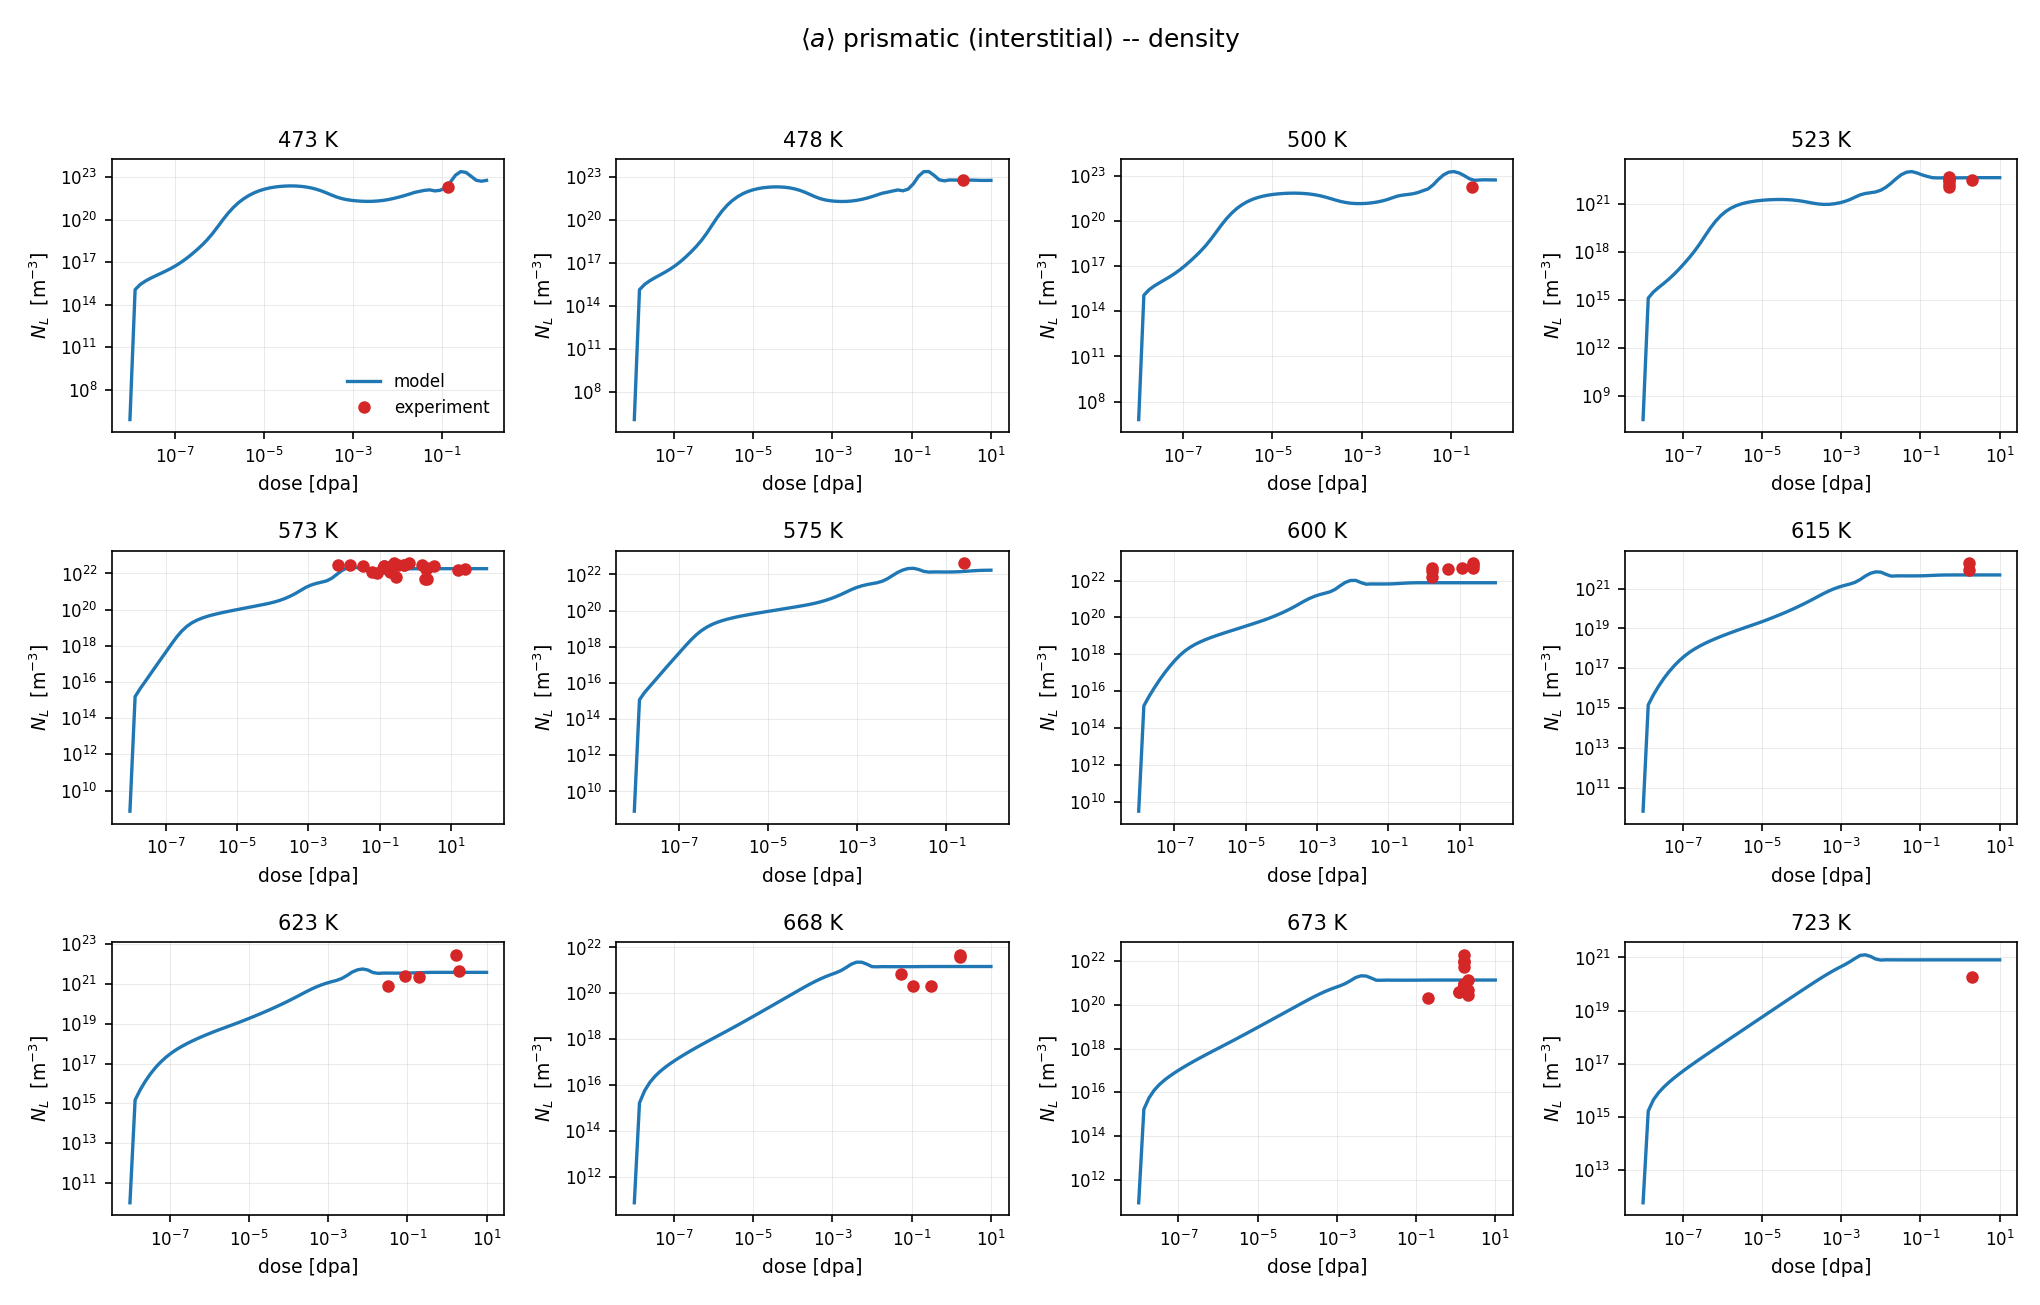
\includegraphics[width=\textwidth]{figures/fit_A_density.png}
\end{minipage}\hfill
\begin{minipage}{0.49\textwidth}\centering
  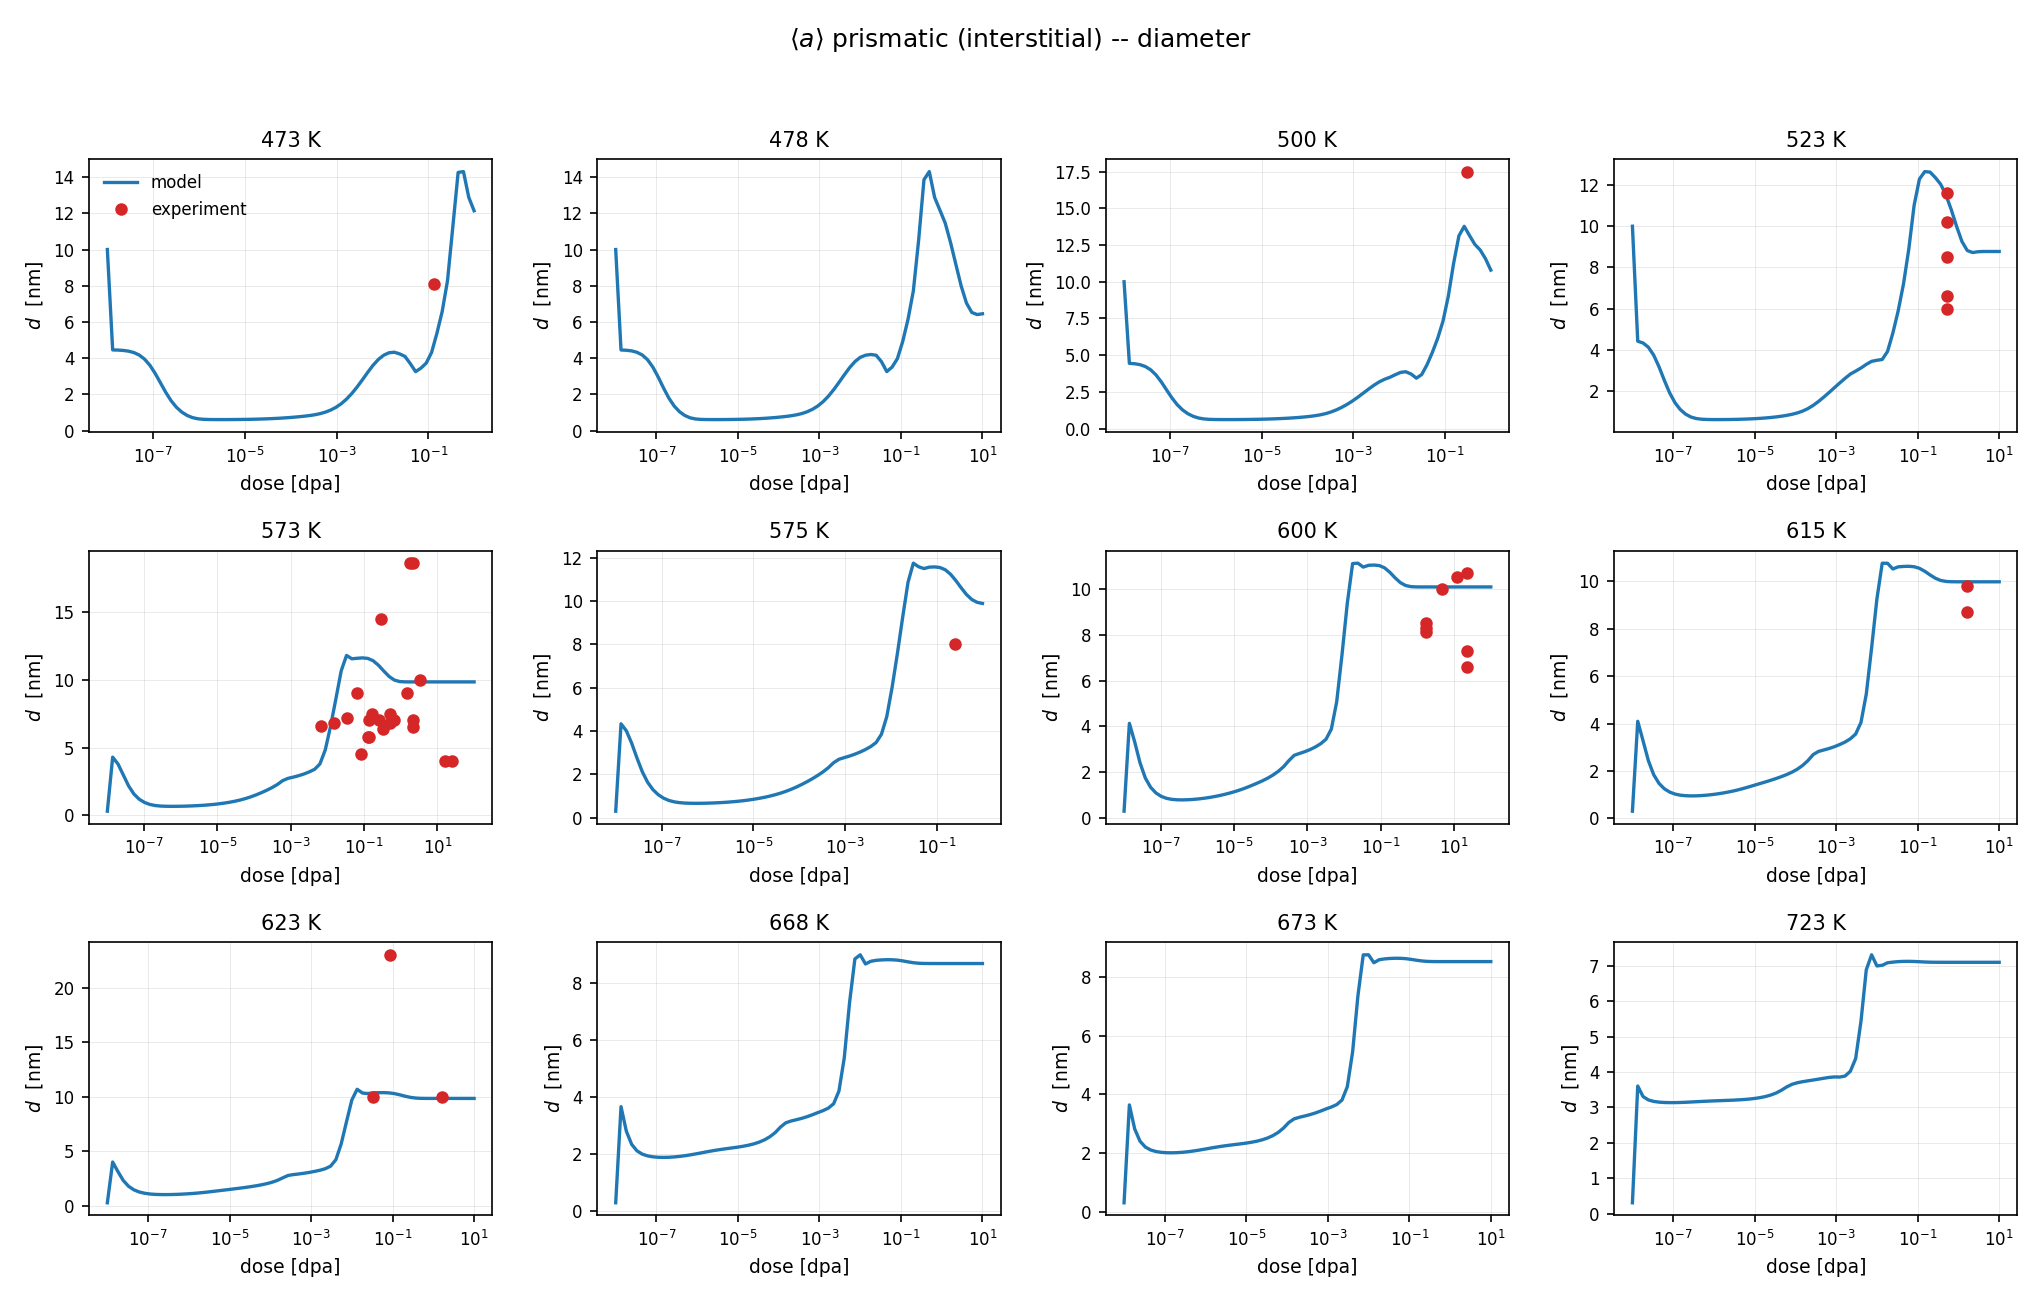
\includegraphics[width=\textwidth]{figures/fit_A_diameter.png}
\end{minipage}
\caption{Prismatic \aloop{} loops by temperature: number density (left) and
mean diameter (right), 71 and 44 points.}
\label{fig:fit-A}
\end{figure}

\begin{figure}[htbp]
\centering
\begin{minipage}{0.49\textwidth}\centering
  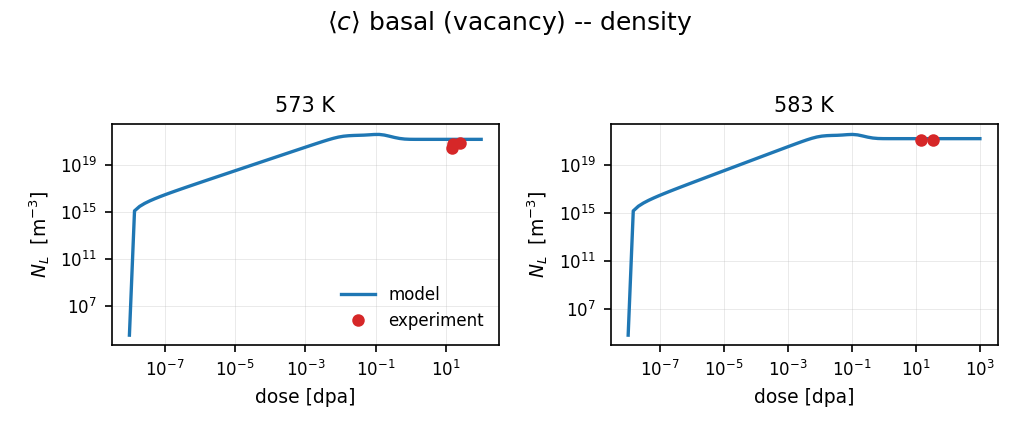
\includegraphics[width=\textwidth]{figures/fit_C_density.png}
\end{minipage}\hfill
\begin{minipage}{0.49\textwidth}\centering
  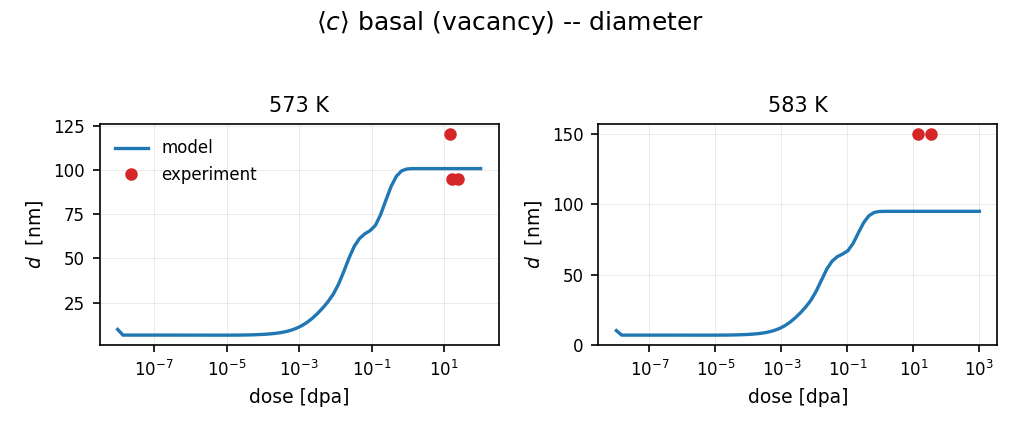
\includegraphics[width=\textwidth]{figures/fit_C_diameter.png}
\end{minipage}
\caption{Basal \cloop{} loops against the five available measurements, all above
14\,dpa; below that the model extrapolates.}
\label{fig:fit-C}
\end{figure}

\begin{figure}[htbp]
\centering
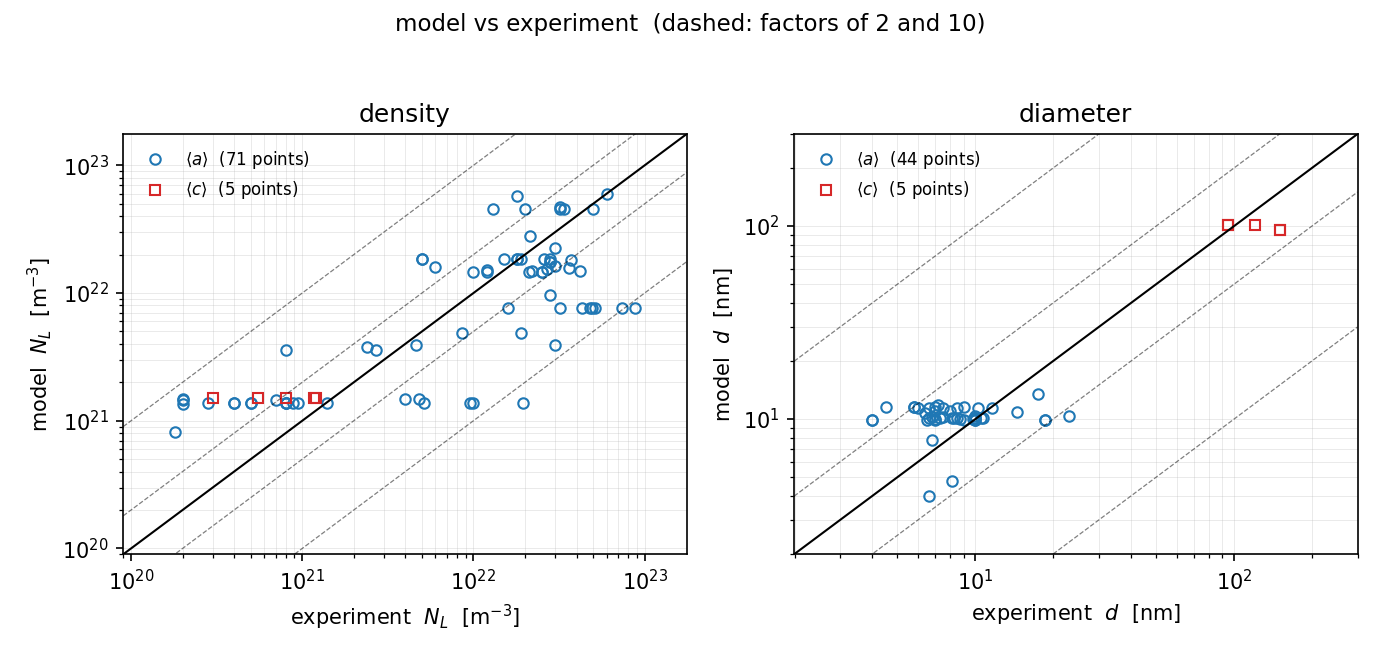
\includegraphics[width=0.62\textwidth]{figures/fit_parity.png}
\caption{Parity plot over all 78 measurements. The diagonal is exact agreement
and the dotted lines a factor of three.}
\label{fig:parity}
\end{figure}

\begin{table}[htbp]
\caption{The calibrated parameter set. The transport anisotropies are
\emph{inputs}, \cref{eq:pinned-pm}, not fitted values. $^{\dagger}$ rests on a
bound and is a constraint rather than an optimum (\cref{sec:bias-caveat});
$^{\ddagger}$ was not moved from the seed.}
\label{tab:fitted}
\centering\small
\begin{tabular}{@{}lr@{\qquad}lr@{\qquad}lr@{}}
\toprule
Parameter & Value & Parameter & Value & Parameter & Value \\
\midrule
\multicolumn{6}{@{}l}{\emph{transport, fixed by \cref{eq:pinned-pm}}}\\
$p^{v}$ & 1.0200 & $p^{i}$ & 0.7000 & $p^{2i}=p^{3i}$ & 0.7000 \\
\midrule
\multicolumn{6}{@{}l}{\emph{calibrated}}\\
$Z^{0}_{v}$ & 1.3000$^{\dagger}$ & $c_{LL}^{a}$ & 4.7720 & $\varepsilon_{2i}$ & 0.0010$^{\dagger}$ \\
$Z^{0}_{i}$ & 0.8935 & $c_{LL}^{c}$ & 1.2386 & $\varepsilon_{3i}$ & 0.007376 \\
$\xi_{c}$   & 2.0000$^{\dagger}$ & $c_{LN}^{a}$ & 94.615 & $\varepsilon_{iL}$ & 0.000200$^{\dagger}$ \\
$Z_N$       & 1.0100$^{\ddagger}$ & $c_{LN}^{c}$ & 1.1198 & $\varepsilon_{vL}$ & 0.005000$^{\dagger}$ \\
$E^{m}_{i}$ (eV) & 0.8970 & $\kappa_{LL}$ & 20.000$^{\dagger}$ & $m^{\mathrm{nuc}}_{a}$ & 53.79 \\
$E^{m}_{2i}$ (eV) & 1.3629$^{\ddagger}$ & $\kappa_{LN}$ & 4.0000$^{\dagger}$ & $m^{\mathrm{nuc}}_{c}$ & 400.00$^{\dagger}$ \\
$E^{b}_{2i}$ (eV) & 0.9570$^{\ddagger}$ & $m_{\min}$ & 5.8286 & $c_{\rho_N}$ & 0.0010$^{\ddagger}$ \\
$\chi$ & 1.0000$^{\ddagger}$ & $m_{\mathrm{vanish}}$ & 14.04 & $k_{\rho_N}^{\mathrm{rec}}$ & $3.5\times10^{-5}$$^{\ddagger}$ \\
 & & $\nu_{\mathrm{vanish}}$ & 0.0010$^{\dagger}$ & & \\
\bottomrule
\end{tabular}
\end{table}

\subsection{What the calibration does not achieve}
\label{sec:atrend}\label{sec:bias-caveat}

The \aloop{} mean conceals the one clear deficiency. Resolved by temperature the
model runs high at both ends and low in the middle:

\begin{center}
\begin{tabular}{@{}lrrrrrrr@{}}
\toprule
$T$ (K) & 473 & 523 & 573 & 575 & 600 & 623 & 673 \\
\midrule
$N_a/N_a^{\exp}$ & 1.29 & 1.66 & 0.88 & 0.35 & \textbf{0.17} & 1.01 & 1.17 \\
$d_a/d_a^{\exp}$ & 0.59 & 1.37 & 1.34 & 1.38 & 1.17 & 0.77 & --- \\
\bottomrule
\end{tabular}
\end{center}

Near $600\,$K the prismatic density is still a factor of six low, and
$573$--$600\,$K is the band \cref{sec:results} runs in. This is not a stage that
failed to converge: four independent searches, seeded differently and carrying
the levers a screen identifies as having the right temperature signature ---
$E^{m}_{i}$, the two coalescence exponents and the cascade partitions
$\varepsilon_{2i}$, $\varepsilon_{3i}$, each of which lowers the low-temperature
end while raising the middle --- all reach the same place, the mean improving
and the middle band not. The deficiency survives the change of anisotropy, the
diameter weighting and its own dedicated stage. Two readings remain, and these
data cannot separate them: the prismatic nucleation term may carry the wrong
temperature dependence, being a cascade partition with none of its own, or the
high-temperature points may not measure the same population, since above
$\sim\!650\,$K the reported \aloop{} loops include vacancy loops --- already the
reason their diameters are excluded from \cref{tab:targets}. The second is
testable by character-resolved measurements at $600$--$700\,$K, and is the more
useful thing to ask of an experiment.

Fixing $p^{m}$ removed four rails and not the pressure that produced them. Four
parameters in \cref{tab:fitted} rest on the edge of the box: $Z^{0}_{v}=1.30$
and the basal sink scale $\xi_{c}=2.00$ at their ceilings, and both coalescence
exponents $\kappa_{LL}=20$, $\kappa_{LN}=4$ at theirs. Their pattern is more
informative than any one of them. $Z^{0}_{v}$ and $\xi_{c}$ both multiply the
basal capture rate and are nearly degenerate, so they are one statement, not
two: given a stated anisotropy the model cannot deliver the measured basal
population without a prefactor no transport argument supplies. That locates the
shortfall in the capture prefactor and not the diffusion tensor. The two
$\kappa$ on their ceilings say the same of coalescence --- the fit wants more
overlap removal than the admissible range allows. That is sharper than the earlier
calibrations supported --- with $p^{v}$ free it absorbed the discrepancy and the
diagnosis stopped at ``the fit wants an implausible anisotropy''; pinned, it
reappears where it cannot be mistaken for transport. Atomistic constraints on
$p^{m}$ would confirm or refute \cref{eq:pinned-pm} directly, and
\cref{eq:Emsplit} would accept them without refitting anything else.

Two caveats on carrying this set into \cref{sec:results}. The fit is the
march's slow step term for term --- one templated function, the same binary and
switches, differing only in whether the mobile species are frozen --- so the
parameters transfer exactly. What does not transfer is what the $0$-D cannot
see: there the vacancy pool is free and re-equilibrates where the march pins it
to the fast solve, and the two need not move a quantity the same way. And the
shifts above target a $3$-D interior not yet re-measured with this set.
